\chapter{Navigation}\label{cha:navigation}
This chapter describes the moving map display as an aid to navigation,
and also describes some of the task and glide related overlays on the
map display.

\section{Map display elements}

\begin{maxipage}
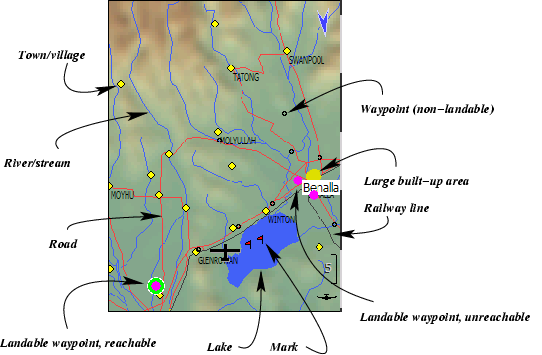
\includegraphics[angle=0,width=0.9\linewidth,keepaspectratio='true']{figures/fig-map.png}
\end{maxipage}

The moving map shows:
\begin{enumerate} 
\item Glider symbol
\item Waypoints
\item The active task
\item The bearing (or route\footnote{The line to the next waypoint may be a {\em route}, as described in Section~\ref{sec:route}.})
  to the next waypoint
\item Special Use Airspace
\item Terrain and topology
\item Markers
\item Trail
\item Glide range\footnote{The glide range is also referred to as the {\em reach}, as described in Section~\ref{sec:reach}.}
\end{enumerate}
The map is drawn in a projected coordinate system (not latitude and
longitude), and the scale can be changed (zooming in and out), as well
as panned.  All navigation functions take the curvature of the Earth
into account.

\section{Glider symbol, map orientation}
The glider symbol shows the position of the glider on the map.  The
orientation of the glider indicates the estimated heading of the
glider.

The map is oriented in one of three ways: North up,
Track up, or Target up.  Configuration settings \config{orientation} can be used
to specify a different map orientation when in circling mode. This is useful to prevent
disorientation when looking at the map while circling.  Target-up when
circling makes it easy to determine which direction to exit the
thermal.

When Track or Target-up is used in circling mode, the glider symbol is
centred on the screen, even if the symbol position is configured differently.
In cruise mode the Track and the Target-up orientation allows the glider
symbol to be positioned (e.g.) 20\% from the bottom of the screen, giving a good view of the
map ahead of the glider.  This position is adjustable in the configuration
\config{gliderposition} settings.

\section{Zoom and map scale}

To change the scale of the map, for PC, PNA, or Pocket PC:
\begin{enumerate}
\item Tap/click on a blank part of the map to highlight the map if it is not
already selected.
Then use mouse wheel, or the Pocket PC up/down key to either zoom
in or out.
\item You can also gesture to change the zoom level. Gesture \gesture{Up/Down}
``Up'' zooms in, ``Down'' zooms out.
\item A PNA with a button wheel let you also change the zoom. 
\item Or select the function from the menus:
\begin{quote}
\bmenu{Display}\blink\bmenu{Zoom In} and \bmenu{Display}\blink\bmenu{Zoom Out}
\end{quote}
\end{enumerate}
On Altair, the rotary knob can be used to zoom in and out.

The map scale is displayed in the lower left corner of the moving map
display. The incicated distance is measured from the left to the right boarder
of the map display.
\marginpar{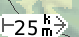
\includegraphics[angle=0,width=0.4\linewidth,keepaspectratio='true']{figures/zoom.png}}

Compaq Aero Users. If you enable the Compaq Aero Game Keys (On the
Q-menu) the centre two front buttons become the up/down keys.

There is a facility to have two zoom settings; one when the glider is
in circling mode, and one in the cruise or final mode.  This is the ``Circling
zoom'' option in the \config{circlingzoom} configuration settings.  
By default, the circling zoom is set to about 2.5 km - 5.0 km, depending on the
display size. When the user zooms in or out, it affects the current
mode's zoom setting only, so when leaving the mode the previous mode's
zoom setting is used.  If ``Circling Zoom'' is not enabled,
there is only a single zoom level.

Auto-zoom automatically zooms in when approaching a waypoint to keep
the waypoint at a reasonable screen distance. When auto-zoom is active,
'AUTO' appears next to the map scale. The user can still zoom
in and out if desired, zoom will be switch to manual control automatically.
\marginpar{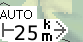
\includegraphics[angle=0,width=0.4\linewidth,keepaspectratio='true']{figures/zoomauto.png}}

To turn auto zoom on or off, select from the menu
\begin{quote}
\bmenu{Display}\blink\bmenu{Display}\blink\bmenu{Zoom Auto} 
\end{quote}

When a waypoint changes (automatically, via the task selector, or by
manually switching waypoints), auto-zoom adjusts the zoom level
automatically so that the next waypoint is visible on the map.

During circling, if a thermal has been detected, then the map is centered about
the thermal or part-way such that the glider is still visible.

\section{Panning the map}

A pan mode allows the user to explore areas beyond the glider.  This
is particularly useful when task planning.
\begin{enumerate}
\item Enable pan mode by pressing 
\begin{quote}
\bmenu{Display}\blink\bmenu{Pan On}
\end{quote}

\item The map can then be panned by dragging the screen or using the cursor
  keys.  For Altair, panning is performed with the inner/outer rotary knob.
\item When done, pan mode has to be disabled manually, by pressing:
\begin{quote}
\bmenu{Pan Off}
\end{quote}

\end{enumerate} 

When pan is active, the text 'PAN' appears next to the map scale.  While
pannig the location of the focus stays in the middle of the display under the
cross hairs.

A special menu of buttons in pan mode is also displayed when in pan
mode.

\begin{center}
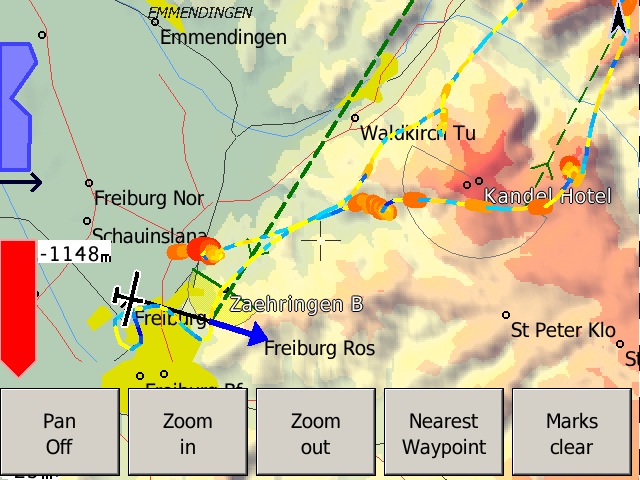
\includegraphics[angle=0,width=0.8\linewidth,keepaspectratio='true']{figures/pan.png}
\end{center}

\section{Waypoints} \label{sec:waypoint-schemes}
Waypoints are displayed with different symbols depending on the
waypoint type; the major distinction being landable and non-landable
waypoints.

The waypoint symbols are drawn as shown below There are three icon sets for
landable waypoints. \config{waypointicons}

\begin{tabular}{c|c|cc|cc|}
Icon set &\begin{sideways}Simple waypoint\end{sideways}
&\begin{sideways}Landable field\end{sideways}
&\begin{sideways}reachable\end{sideways}
&\begin{sideways}Aerfield\end{sideways}
&\begin{sideways}reachable\end{sideways}\\
\hline
Purple Circle &

\includegraphics[width=0.5cm]{icons/map_turnpoint.pdf} &

\includegraphics[width=0.8cm]{icons/winpilot_landable.pdf} &

\includegraphics[width=0.8cm]{icons/winpilot_reachable.pdf} &
\colorbox{white}{
\includegraphics[width=0.8cm]{icons/winpilot_landable.pdf}}
& 
\includegraphics[width=0.8cm]{icons/winpilot_reachable.pdf} \\
\hline
B/W Icon & 

\includegraphics[width=0.5cm]{icons/map_turnpoint.pdf} &

\includegraphics[width=0.9cm]{icons/alt_landable_field.pdf} &

\includegraphics[width=0.9cm]{icons/alt_reachable_field.pdf} &
\colorbox[rgb]{0.94,0.94,0.94}{
\includegraphics[width=0.9cm]{icons/alt_landable_airport.pdf}}
& 
\includegraphics[width=0.9cm]{icons/alt_reachable_airport.pdf} \\
\hline
Orange Icon & 

\includegraphics[width=0.5cm]{icons/map_turnpoint.pdf} &

\includegraphics[width=0.9cm]{icons/alt2_landable_field.pdf} &

\includegraphics[width=0.9cm]{icons/alt_reachable_field.pdf} &
\colorbox{white}{
\includegraphics[width=0.9cm]{icons/alt2_landable_airport.pdf}}
& 
\includegraphics[width=0.9cm]{icons/alt_reachable_airport.pdf} \\
\hline
\end{tabular}


Waypoints are optionally labelled according to one of several
abbreviation schemes\config{labels} and visibility \config{labelvisibility}.

XCSoar continually calculates which landing points are within gliding
range using the current wind estimate.  The estimated arrival altitude
{\em above the arrival safety height} of reachable landable points is
displayed next to the waypoint.  This arrival altitude is calculated
with the glider performance and MacCready setting configurable as
either that of the task\config{reachpolar}, or at a safety MacCready value.

\section{Active task}

The active task course is drawn on the map as a green dashed line.
Assigned area tasks also show the task sectors or areas as a yellow shaded
region.  
Circles are always drawn around start and finish points, lines are
only drawn if the start/finish points are of line type.  Task
observation sectors are drawn as segments.

At all times a thick black line is drawn from the glider to the next
waypoint in the task.  This line may be the direct path to the waypoint,
or may be a {\em route} path clearing terrain and airspace obstacles, described in
further detail in Section~\ref{sec:route}.

\begin{center}

\begin{tabular}{c c c}
{\it Start/finish} & {\it Sector} & {\it Cylinder} \\
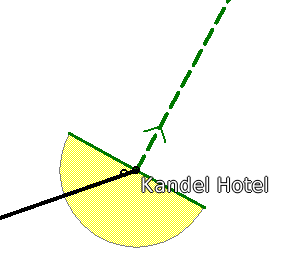
\includegraphics[angle=0,width=0.3\linewidth,keepaspectratio='true']{figures/cut-startfinish.png} &
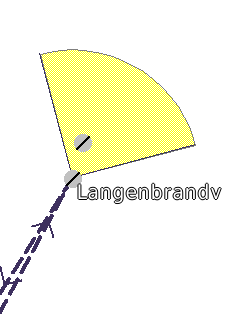
\includegraphics[angle=0,width=0.3\linewidth,keepaspectratio='true']{figures/cut-sector.png} &
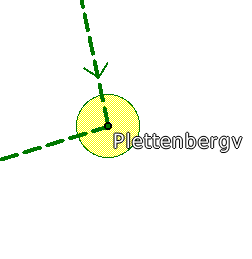
\includegraphics[angle=0,width=0.3\linewidth,keepaspectratio='true']{figures/cut-barrel.png} \\
\end{tabular}
\end{center}

\section{Terrain and Topology}

The following topological features are drawn on the map:
\begin{itemize}
\item Major roads, shown as red lines
\item Rivers, shown as blue lines
\item Large water bodies (lakes), shown as blue areas
\item Large cities, shown as yellow areas
\item Small population areas, shown as yellow diamonds
\end{itemize}
Cities and small population areas are labeled in italics.

Terrain is coloured according to height, and optionally shaded by sun
direction or lift-generating slope.  Invalid terrain, or terrain below
sea level is coloured blue.

Terrain is shaded to improve visibility.  Currently the shading
is set up so that the virtual lighting position is the wind bearing,
thus brighter areas are on the upwind side of hills and dark areas in
the lee of the hill.  The amount of shading and overall terrain
brightness is configurable.  Support for a sun ephemeris is underway.
Terrain shading and brightness can be configured \config{shading}.

Both terrain and topology display can be switched on or off from the
menu:
\begin{quote}
\bmenu{Display}\blink\bmenu{Display}\blink\bmenu{Terrain On} \\
\bmenu{Display}\blink\bmenu{Display}\blink\bmenu{Topology On}
\end{quote}

\begin{center}
\begin{tabular}{c c}
Topology & Terrain \\
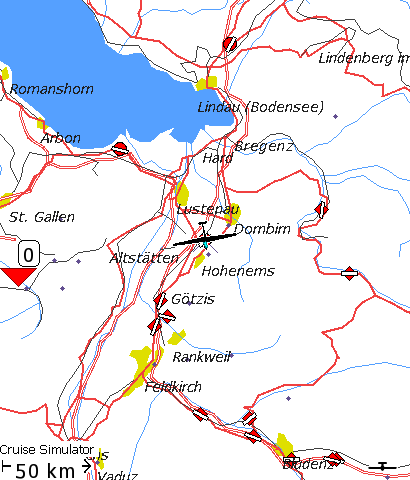
\includegraphics[angle=0,width=0.4\linewidth,keepaspectratio='true']{figures/cut-topo.png} &
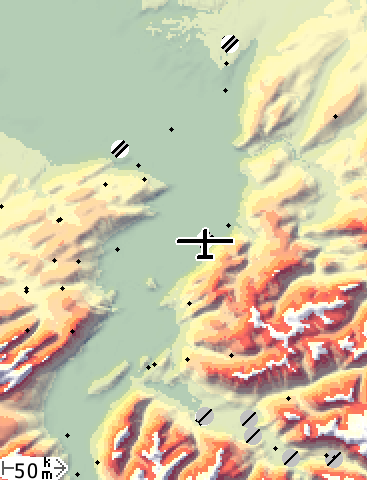
\includegraphics[angle=0,width=0.4\linewidth,keepaspectratio='true']{figures/cut-terrain.png} \\
\end{tabular}

\end{center}

If the terrain data is not available (or terrain display is turned
off), the background colour of the map window is white.  All terrain
below mean sea level is coloured blue.  If you are flying outside the
terrain region, the background colour will be white.

The screen can be de-cluttered, turning off the display of topology
labels and non-task waypoint labels by toggling:
\begin{quote}
\bmenu{Display}\blink\bmenu{Display}\blink\bmenu{Labels Off}
\end{quote}


\section{Trail}\label{sec:trail}

An optional 'snail trail' is drawn on the map showing the glider's
path history.  The colour and thickness of the trail depends on the height or
on the variometer value. \config{snailtype} 

\begin{center}
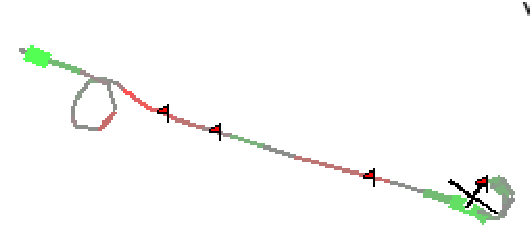
\includegraphics[angle=0,width=0.8\linewidth,keepaspectratio='true']{figures/snail.pdf}
\end{center}

If Vega or an intelligent variometer is connected with Netto output,
the Netto vario value is used; hence the colours and thickness of the
trail indicates the air-mass vertical movement rather than the glider's
vertical movement	.

The snail trail display can be toggled between off, a short trail
(about ten minutes), a long trail (about one hour) or a full trail
which displays the entire flight.  This can be performed permanently
through the configuration \config{snailtrail} settings or temporarily by the
menu:
\begin{quote}
\bmenu{Display}\blink\bmenu{Display}\blink\bmenu{Snail trail}
\end{quote}

Note that for all of these modes, the snail trail is short in
circling mode in order to reduce screen clutter.

In order to assist centering thermals in the presence of wind, the
snail trail can be artificially drifted with the wind as it is
displayed (this is drift compensation).  In this way, the snail trail
is referenced to the prevailing wind rather than referenced to the
ground.  Since thermals drift with the wind also, the drifted trails
give a better indication of where the glider has been relative to the
thermals.

An example of this is illustrated below.  Note that when trail drift
compensation is active (right picture), the glider appears to be
circling in a column rather than an elongated spiral (left picture).

\begin{center}
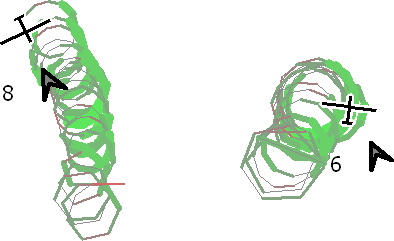
\includegraphics[angle=0,width=0.8\linewidth,keepaspectratio='true']{figures/traildrift.png}
\end{center}

Enabling trail drift compensation is performed through the
configuration settings \config{traildrift}.  The compensation is only performed
whilst in circling mode; the display of the trail in cruise mode is unaffected.
This can also be performed from the wind settings dialog:
\begin{quote}
\bmenu{Config}\blink\bmenu{Setup Wind}
\end{quote}

The trail drift display is useful also to show more clearly when thermals
are cranked due to wind shear.

The trail width can be adjusted in the configuration settings \config{trailwidth}.

\section{Markers}

\begin{tabular}{c}%{c}

\includegraphics[angle=0,width=0.75cm,keepaspectratio='true']{icons/map_flag.pdf}\\
(a)
\end{tabular}


Markers are shown as small flags (a) on the map.  The markers can be dropped
manually, by pressing a button, or automatically.  An example use of
automatic markers is to drop markers when entering circling mode, as a
simple way of showing all thermals encountered.

Markers are not preserved after XCSoar is exited, however the location
of all marks are appended to the file \verb|xcsoar-marks.txt|.

Markers are dropped by the menu, or by gesture \gesture{Left}: 
\begin{quote}
\bmenu{Display}\blink\bmenu{Mark Drop}
\end{quote}

\section{Glide range line}\label{sec:reach}

A reachable glide `footprint' is displayed on the map display as a
black and white dashed line, indicating where the glider would descend
through the terrain clearance height.  The reach shows clearance
tracks extending in all directions, optionally including paths around
terrain obstructions.  This feature is useful in assessing range with
respect to topology when searching low for lift, and when flying in
mountainous areas.

Reach calculations may be configured \config{turningreach} to two levels of detail:
\begin{description}
\item[Straight line] If turning reach is disabled, then the reach shows the
 furthest distance the glider can fly in final glide in all directions without
 turning.  This reach appears as a closed ring around the glider.

\begin{center}
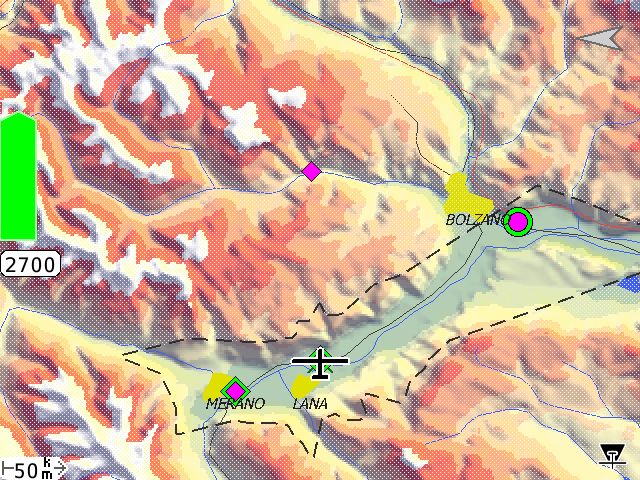
\includegraphics[angle=0,width=1.0\linewidth,keepaspectratio='true']{figures/reach1.png}
%{\it DIAGRAM CUTOUT SHOWING GLIDE RANGE FOOTPRINT.  NO TOPOLOGY,
%FULLSCREEN, NO TASK. TURNING=FALSE}
\end{center}

\item[Turning] If turning reach is enabled, then the reach shows the
  greatest area the glider can reach in all directions, even allowing
  turns around obstructions.\footnote{The maximum number of turns is
    set to three, and no turns may be greater than 90 degrees.}  The
  reach area appears as a closed ring around the glider but may also
  include holes indicating mountain peaks that the glider cannot reach
  without further climb.

\begin{center}
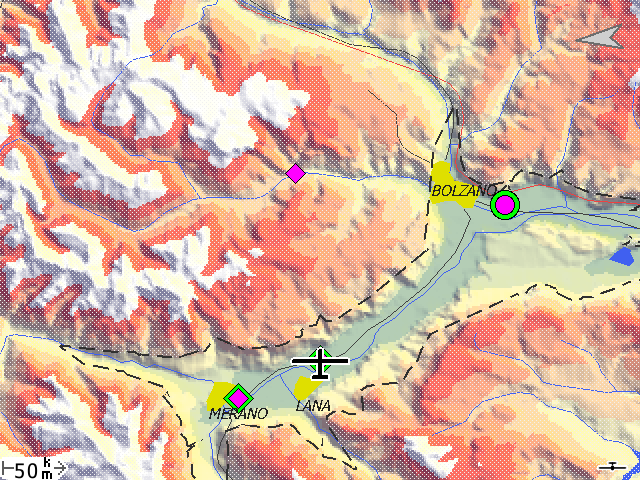
\includegraphics[angle=0,width=1.0\linewidth,keepaspectratio='true']{figures/reach2.png}
%{\it DIAGRAM CUTOUT SHOWING GLIDE RANGE FOOTPRINT.  NO TOPOLOGY,
%FULLSCREEN, NO TASK. TURNING=TRUE}
\end{center}

\end{description}

The display can be configured to additionally blur the unreachable area
outside the glide range. \config{gliderange}
The final glide path is checked for whether the glider clears terrain along
the path by the terrain clearance height.  If clearance is not attained, a red
cross appears on the map at the point where the violation occurs. If a target is
defined the calculation is done along the path to the target. 

If reach is enabled, then the reachability of landable waypoints is used
by the abort task mode, alternate landable option lists and display of
landable waypoints on the map.

Note that task calculations are otherwise unaffected by reach
calculations --- for example, heights required as shown in the final
glide bar or task data as displayed in infoboxes do not take reach into account.

Furthermore, the reach calculations are used for footprint, landable
waypoint arrival heights, abort mode and the alternates dialog.  The glider
performance and MacCready setting used in these calculations are configurable\config{reachpolar}:
\begin{description}
\item[Task] The MC value is that used in the task.
\item[Safety MC] A configurable, typically low MC value is set by the user to set
 performance near, but slightly degraded to, best glide performance.

\end{description}

\section{Status dialog}\label{sec:aircr-stat-dial}

The nearest landmark function, typically available via the button
menu, brings up a status message describing the name, distance and
bearing to the nearest landmark.  The nearest landmark is also
reported on the status dialog.

You may find this function useful when you need to report your
location to others.

Currently the landmarks scanned are the list of waypoints.  In the
future, XCSoar may also search for nearby towns and cities in the
topology database.

The aircraft status dialog (see Section~\ref{sec:dialog-windows})
shows the status of the aircraft's locality, and can be useful when
giving position reports.

This is accessed via the menu under: 
\begin{quote}
\bmenu{Info}\blink\bmenu{Info}\blink\bmenu{Status}.
\end{quote}
and then selecting the page `Aircraft'.

\section{Route}\label{sec:route}

XCSoar can plan paths around terrain and airspace obstacles in three
dimensions from the aircraft to the destination.  Such a path is known
as a route.  The height of the destination is the arrival height for
final waypoints, or may be higher for intermediate waypoints, as
dictated by the task system as required to complete the task.  Route
planning functions in normal ordered task mode, abort mode and goto
mode.

\begin{center}
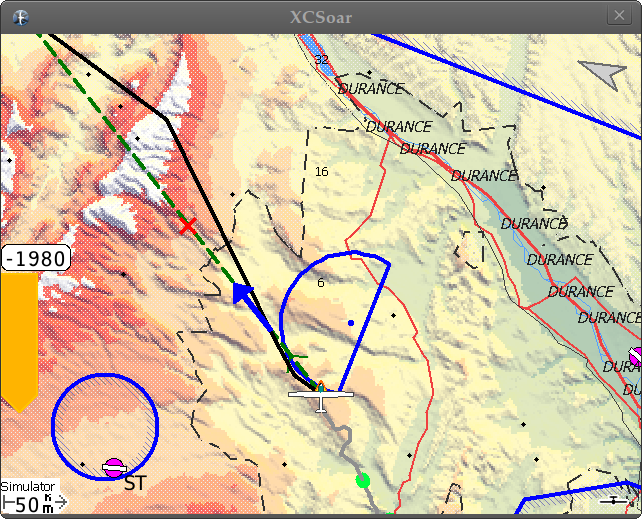
\includegraphics[angle=0,width=1.0\linewidth,keepaspectratio='true']{figures/route3.png}
\end{center}

Routes take into account the glider polar performance and are
calculated to be optimal in the sense of minimum time.  By default,
route calculation is disabled, and can be enabled for terrain only or
terrain and airspace avoidance \config{routemode}.

Terrain is avoided vertically by the terrain safety height
\config{safetyterrain}, with no additional lateral clearance imposed.
Valid routes may result in the aircraft arriving at the destination
higher than the minimum height --- such as can occur when the
destination is just beyond a steep mountain.

Airspace is avoided horizontally by a buffer of approximately 250 m,
with no additional vertical clearance imposed.  Valid routes may fly
below or above airspace.

If MacCready is positive, then climbs are optionally allowed
\config{routeceiling} in the computed routes.  The top of the climb
may be limited to 500 m above the heigher of the start and destination
ceiling, or increased to the ceiling defined by the thermal ceiling
\config{routeceiling}.  Climbs above the higher of the start and
destination altitude are penalised by a slower climb rate than the
actual MacCready value.

Some approximations and limitations of the route planning system are as follows:
\begin{itemize}
\item Where climbs are necessary (and permitted) to reach the destination,
the climbs are assumed to occur at the start of the route.
\item Climb-cruise segments are assumed to occur at constant altitude,
equivalent to many small climbs distributed along the path.
\item Individual turns between path segments greater than 90 degrees
  are not permitted.
\item Failures of the solver result in the route reverting to direct flight
from the aircraft location to the destination.
\end{itemize}

